\documentclass[11pt,a4paper]{article}
\usepackage[margin=25mm]{geometry}
\usepackage[utf8]{inputenc}
\usepackage[T1]{fontenc}
\usepackage{lmodern}
\usepackage{amsmath,amssymb,bm}
\usepackage{graphicx}
\usepackage{booktabs}
\usepackage{caption}
\usepackage{subcaption}
\usepackage{natbib}
\usepackage{setspace}
\usepackage{lineno}
\usepackage[hidelinks]{hyperref}
\usepackage{microtype}
\usepackage{xcolor}
\usepackage{adjustbox}
\graphicspath{{figures/}}
\captionsetup{font=small,labelfont=bf,justification=justified}
\DeclareMathOperator*{\argmax}{arg\,max}
\DeclareMathOperator{\median}{median}
\DeclareMathOperator{\logit}{logit}
\DeclareMathOperator{\Gap}{Gap}
\newcommand{\bS}{\mathbf{S}}
\onehalfspacing
\linenumbers

\title{Clustering trajectories of modelled estimates: an uncertainty aware framework, with an application to global cardiovascular disease burden, 1990 to 2023}
\author{Eben Afrifa-Yamoah\thanks{School of Science, Edith Cowan University, Perth, Western Australia. Mathematical Applications and Data Analytics; Centre for Marine Ecosystems Research. Correspondence: e.afrifayamoah@ecu.edu.au. ORCID 0000-0003-1741-9249.}}
\date{Draft v1.0, 3 October 2026}

\begin{document}
\maketitle

\begin{abstract}
\noindent Modelled health estimates such as those of the Global Burden of Disease (GBD) study are increasingly treated as data in secondary analyses, including trajectory clustering, that were designed for observed values. Such analyses inherit no uncertainty from the estimates, choose the number of clusters by criteria blind to it, and assign every unit with the same confidence whether its series rests on vital registration or on covariates. We propose an uncertainty aware framework for clustering trajectories of modelled estimates and show that it changes the answer. The framework separates each trajectory into a level and a shape so that clusters describe form rather than magnitude; derives a membership probability for every unit by perturbing the series within its published uncertainty and reclustering; chooses the number of clusters by stability under that uncertainty rather than by geometric fit; and attributes membership to development level, region and measurement quality. Applied to age-standardised cardiovascular disease DALY rates for 201 countries from 1990 to 2023 (GBD 2023), the framework selects two clusters where the gap statistic selects three; the third cluster's median membership probability is 0.70 and it does not survive the estimates' own uncertainty. The two retained clusters had indistinguishable burden in 1990 (median 7,239 versus 7,062 per 100,000) and diverged only in trajectory: a stalled group of 78 countries (median change $-8\%$, 40 of them in sub-Saharan Africa) and a sustained decline group of 92 countries ($-52\%$, including the whole high-income super region). Thirty-one countries with membership probability below 0.70 are reported as unassigned; a multinomial model shows they concentrate at the development level where the two-shapes overlap. The partition is reproduced exactly on death rates, on a 2000 to 2023 window, and under country bootstrap resampling. Restricting to the half of countries with the narrowest published intervals, which excludes almost all of sub-Saharan Africa, reveals a third, well-supported trajectory type among the former Soviet and Eastern European countries that the pooled analysis absorbs into the decline cluster, and interval width predicts stalled membership beyond development level. We conclude that stability under published uncertainty, and an explicit account of measurement quality, should be routine in any clustering of modelled estimates. R code reproduces every result from the public GBD outputs.

\medskip\noindent\textbf{Keywords:} trajectory clustering; uncertainty propagation; cluster stability; Global Burden of Disease; cardiovascular disease; modelled estimates
\end{abstract}

\section{Introduction}

Countries do not move through the cardiovascular transition together. In high-income countries the fall in cardiovascular mortality that began in the 1970s has slowed since the early 2010s and, in some younger age groups, reversed \citep{lopez2019,dowd2025}. Elsewhere the age-standardised burden continued to rise long after it had peaked in the West and has only recently turned down in many places; globally, cardiovascular disease still caused 19.2 million deaths and 437 million DALYs in 2023, with a sixteenfold spread in age-standardised DALY rates between countries \citep{gbdcvd2025}. Which countries share a trajectory, and whether those groupings follow geography, development level, or neither, is a natural question for cluster analysis. The GBD study, with annual estimates for 204 countries and territories from 1990 onward \citep{gbd2023dalys,gbd2023cod}, is the obvious source of data.

The difficulty is that GBD values are not observations. They are outputs of a modelling pipeline that combines vital registration, verbal autopsy, surveys, and covariates, and for many countries the covariates carry most of the weight. GBD rates the underlying cause-of-death data on a zero-to-five-star scale; in GBD 2016, 27 countries had no vital registration or verbal autopsy data at all and 44 more sat at the lowest non-zero rating \citep{gbd2016cod}. Every estimate is published with a 95\% uncertainty interval taken from 1,000 posterior draws, and those intervals are wide precisely where the primary data are thin. Commentators have begun to ask that users of GBD outputs assess the certainty of the estimates before building on them \citep{munozlaguna2024}; this paper is a methodological answer to that request for one common kind of secondary analysis.

Secondary analyses that cluster GBD trajectories have so far treated the point estimates as the data. A recent global study clustered joint HIV and tuberculosis mortality trajectories for 204 countries on point estimates alone \citep{hivtb2025}, and the same practice runs through the growing literature that applies trajectory methods to GBD series. Three things then go unexamined. The number of clusters is chosen by geometric criteria such as the silhouette \citep{rousseeuw1987} or the gap statistic \citep{tibshirani2001}, which know nothing about how far each point could move. Every country is assigned with equal confidence. And a cluster that exists because several poorly-measured series happen to share a smooth modelled shape cannot be told apart from one that reflects a shared epidemiological reality.

Statisticians have long argued that cluster solutions should be checked for stability. Hennig's cluster-wise assessment resamples the units and asks whether each cluster reappears \citep{hennig2007}; the same idea underlies bootstrap selection of the number of clusters \citep{fang2012} and the stability tools in longitudinal clustering software \citep{denteuling2024}. Simulation studies confirm that measurement error can create or destroy clusters depending on the algorithm \citep{measerr2020}. What these approaches resample is the set of units. When every unit's value carries its own published uncertainty, the natural quantity to resample is the value, and that is the step taken here. We also show, by running the two schemes side by side, where resampling values and resampling units agree and where they part company.

This paper makes three contributions. It assembles a framework for clustering trajectories of modelled estimates that carries the published uncertainty through to membership and to the number of clusters, and sets it out with enough formality to be reimplemented. It applies the framework to global cardiovascular disease burden and shows that a conventional criterion returns a cluster the data cannot support, that two groups with identical burden in 1990 separate cleanly on trajectory shape, and that the partition is reproduced across burden measures, analysis windows and resampling schemes. And it uses the width of the published interval as a measure of how much each country's series depends on modelling, showing that the stalled trajectory is concentrated among weakly-measured countries and that the well-measured subset carries a richer structure than the pooled analysis reveals. All code is in R and reproduces every number from the public GBD outputs.

Section~\ref{sec:data} describes the data and how they were obtained. Section~\ref{sec:methods} develops the framework, giving for each component the decision it embodies, the alternatives considered, and the reason for the choice. Section~\ref{sec:results} reports the case study and its robustness checks. Section~\ref{sec:discussion} discusses what the framework changes, where it falls short, and what the cardiovascular result does and does not show.

\section{Data}\label{sec:data}

The primary series is the age-standardised rate of disability-adjusted life years (DALYs) per 100,000 for cardiovascular diseases (GBD level-2 cause), both sexes, in each of 204 countries and territories for every year from 1990 to 2023, from GBD 2023 \citep{gbd2023dalys}. DALYs combine fatal and non-fatal burden and are the measure GBD leads with; the age-standardised death rate for the same cause, years and countries was obtained for a sensitivity analysis. Age standardisation uses the GBD world standard population and is essential for comparing trajectories across countries, since a rising crude rate in an ageing population can coincide with a falling age-standardised one.

Covariates were the Socio-demographic Index (SDI) for 2023, a composite of income per capita, mean years of schooling and fertility under 25 on a zero to one scale \citep{gbd2023dalys}; the GBD super region (seven groups); and the World Bank income group used to partition the extraction. Country centroids for the spatial analysis were taken from the largest polygon of each country in the \texttt{maps} package for R.

\subsection{Access and processing}

All GBD values were retrieved programmatically through the IHME GBD 2023 Model Context Protocol connector rather than from the GBD Results Tool, and the route shaped the analysis in two ways. The connector caps each response at roughly 667 location years for DALYs and 476 for deaths in its default format, so each global series was assembled from 12 calls, one per World Bank income group and year window, and reconciled to 203 countries with 34 complete years. The connector also supplies the 95\% interval for the all-ages rate but not for the age-standardised rate, and does not expose the posterior draws; the uncertainty propagation in Section~\ref{sec:stability} therefore rests on an approximation described there, and a draw-level replication from the Results Tool export remains the first item for revision.

The analysis set is 201 countries: the 204 GBD locations less Hong Kong and Macao, which are World Bank economies but sit under China in the GBD hierarchy, and Tuvalu, which lacks an income classification in the connector and a polygon in the base map. All rates were log transformed before analysis.

\section{Methods: an uncertainty aware framework}\label{sec:methods}

The framework has four components, applied in sequence. Each is described with the decision it embodies, the alternatives we considered, and why we chose as we did. The guiding principle is that every quantity the framework reports, including the number of clusters, should have been tested against the uncertainty that the data provider published.

\subsection{Notation and inputs}

Let $i = 1, \ldots, n$ index countries and $t = 1, \ldots, T$ index years, with $n = 201$ and $T = 34$. For each country year, GBD publishes a point estimate $r_{it}$ of the age-standardised rate and a 95\% uncertainty interval $[\ell_{it}, u_{it}]$ obtained as the 2.5th and 97.5th percentiles of 1,000 posterior draws. We work throughout on the log scale, $y_{it} = \log r_{it}$, because rates are strictly positive, their uncertainty is approximately symmetric on that scale, and differences in $y$ are proportional changes that compare across countries with very different burden. The published interval is converted to a per-observation standard deviation on the log scale by treating the posterior of $r_{it}$ as log-normal,
\begin{equation}\label{eq:sd}
s_{it} = \frac{\log u_{it} - \log \ell_{it}}{2\, z_{0.975}}, \qquad z_{0.975} = 1.96.
\end{equation}
Equation~\eqref{eq:sd} recovers the posterior standard deviation exactly if the draws are log-normal and approximately otherwise. It is the only information about uncertainty the framework needs, and it is available for every GBD output. Its country mean,
\begin{equation}\label{eq:width}
w_i = \frac{1}{T}\sum_{t=1}^{T} s_{it},
\end{equation}
is used in Section~\ref{sec:attribution} as a measure of how far country $i$'s series depends on modelling rather than on primary data.

\subsection{Level and shape}

A trajectory has a magnitude and a form, and clustering on the raw series conflates them: two countries with the same decline but burden differing threefold sit far apart, while a high burden country that is stalling can sit next to one that is falling fast. We separate the two by an orthogonal decomposition of each series into a level and a shape,
\begin{equation}\label{eq:decomp}
y_{it} = L_i + S_{it}, \qquad L_i = \frac{1}{T}\sum_{t=1}^{T} y_{it}, \qquad S_{it} = y_{it} - L_i,
\end{equation}
so that $\sum_t S_{it} = 0$ for every country. The shape vector $\bS_i = (S_{i1}, \ldots, S_{iT})^\top$ is the log ratio of the rate in each year to the country's own average over the period; it is dimensionless, proportional, and invariant to any constant rescaling of the series. Clustering uses $\bS_i$ alone, and $L_i$ is kept as a diagnostic.

Two alternatives were considered. First differences, $\Delta y_{it} = y_{it} - y_{i,t-1}$, remove level and any constant trend and leave acceleration; in these data they gave a silhouette of 0.09 at $k = 2$ and no interpretable structure, because most of the signal is in the trend itself. Fitting each series with a low-order polynomial or B spline and clustering the coefficients is attractive for noisy series but adds a tuning choice and, with 34 annual points and smooth GBD trajectories, offered no reduction worth the cost. Mean centring is the simplest option that isolates form, and we check after clustering that it worked. For a partition $\mathcal{C} = \{C_1, \ldots, C_k\}$ with $c(i)$ the cluster of country $i$, the share of level variance explained by membership,
\begin{equation}\label{eq:r2level}
R^2_L = 1 - \frac{\sum_i \bigl(L_i - \bar L_{c(i)}\bigr)^2}{\sum_i \bigl(L_i - \bar L\bigr)^2},
\end{equation}
should be near zero, and the adjusted Rand index \citep{hubert1985} between $\mathcal{C}$ and the tertiles of $L$ should be near zero.

\subsection{Clustering}

Shape vectors are clustered by agglomerative hierarchical clustering with Ward's criterion on Euclidean distance $d(i,j) = \lVert \bS_i - \bS_j \rVert_2$. At each step Ward's method merges the pair of clusters $A$ and $B$ whose union least increases the total within-cluster sum of squares,
\begin{equation}\label{eq:ward}
\Delta(A, B) = \frac{|A|\,|B|}{|A| + |B|}\, \lVert \bar{\bS}_A - \bar{\bS}_B \rVert_2^2,
\end{equation}
where $\bar{\bS}_A$ is the centroid of $A$. We use the \texttt{ward.D2} implementation, which applies the criterion to squared distances as Ward intended \citep{murtagh2014}. Ward's method produces compact groups of roughly equal variance and a full dendrogram, so the partition $\mathcal{C}_k$ for every $k$ comes from one tree by cutting at $k$ branches, which simplifies the stability analysis. The partition was checked against partitioning around medoids at the same $k$; agreement was moderate (adjusted Rand index 0.72 at $k = 2$), which is expected when a share of countries sit near a boundary and is one reason to report membership probabilities rather than hard labels.

Euclidean distance on centred series treats every year equally and cannot align two countries whose transition occurs at different dates. Dynamic time warping would allow that alignment; we did not use it because the timing of a country's turning point is itself of interest and warping removes it. A codispersion based dissimilarity, which measures co variation of two series at a chosen lag rather than pointwise distance \citep{fouedjio2026}, is a promising alternative for regionalised series and is left for future work.

\subsection{Membership probability and the number of clusters}\label{sec:stability}

This component makes the framework uncertainty aware, and it rests on one observation: each $y_{it}$ comes with a published interval, so the natural perturbation is of the value, not of the sample of countries. For $b = 1, \ldots, B$ we draw a perturbed panel
\begin{equation}\label{eq:perturb}
y^{(b)}_{it} = y_{it} + s_{it}\,\varepsilon^{(b)}_{it}, \qquad \varepsilon^{(b)}_{it} \overset{\text{iid}}{\sim} \mathcal{N}(0,1),
\end{equation}
recompute level and shape by~\eqref{eq:decomp}, and recluster at the same $k$ to obtain a perturbed partition with labels $c^{(b)}(i)$. Because cluster labels are arbitrary, each perturbed partition is aligned to the reference by majority overlap: perturbed cluster $m$ is mapped to the reference cluster it shares most members with,
\begin{equation}\label{eq:align}
\sigma^{(b)}(m) = \argmax_{c \in \{1,\ldots,k\}} \bigl| C^{(b)}_m \cap C_c \bigr|.
\end{equation}
The membership probability of country $i$ is the share of draws in which it returns to its reference cluster under that alignment,
\begin{equation}\label{eq:pmember}
p_i = \frac{1}{B}\sum_{b=1}^{B} \mathbf{1}\Bigl\{ \sigma^{(b)}\bigl(c^{(b)}(i)\bigr) = c(i) \Bigr\}.
\end{equation}
We used $B = 1{,}000$. The map~\eqref{eq:align} is many to one, so two perturbed clusters can be sent to the same reference cluster; this is deliberate, since a reference cluster that splits under perturbation should register as unstable for the members that leave, and it does.

Three decisions follow from~\eqref{eq:pmember}. A country is reported as assigned only if its membership probability clears a threshold $\tau$,
\begin{equation}\label{eq:assign}
a_i = \begin{cases} c(i) & \text{if } p_i \geq \tau, \\ 0 & \text{otherwise,} \end{cases} \qquad \tau = 0.70,
\end{equation}
where $a_i = 0$ denotes unassigned; $\tau$ is in the range Hennig recommends for a stable cluster under resampling \citep{hennig2007}, and the number of unassigned countries is reported. The number of clusters is the largest $k$ for which every cluster is stable on its own terms,
\begin{equation}\label{eq:kstar}
k^{*} = \max\Bigl\{ k : \min_{c \in \{1,\ldots,k\}} \median_{i \in C_c}\, p^{(k)}_i \geq \pi \Bigr\}, \qquad \pi = 0.80,
\end{equation}
with $p^{(k)}_i$ computed under the $k$-cluster partition. This is deliberately conservative relative to the two conventional criteria reported alongside it. The silhouette \citep{rousseeuw1987} rewards separation of point estimates. The gap statistic \citep{tibshirani2001} compares the log pooled within-cluster dispersion $W_k = \sum_c \sum_{i \in C_c} \lVert \bS_i - \bar{\bS}_c \rVert_2^2$ with its expectation under a uniform reference,
\begin{equation}\label{eq:gap}
\Gap(k) = \mathbb{E}^{*}\bigl[\log W_k\bigr] - \log W_k,
\end{equation}
and selects the smallest $k$ with $\Gap(k) \geq \Gap(k+1) - \hat\sigma_{k+1}$, the expectation and its standard error coming from 100 reference sets. Neither criterion knows how far each point could move; \eqref{eq:kstar} does, and can reject a partition that \eqref{eq:gap} accepts.

The same machinery runs with units resampled instead of values. In the country bootstrap, draw $b$ takes a bootstrap sample of countries, clusters the unique members, and aligns as in~\eqref{eq:align}; $p_i$ is then the share of the draws containing $i$ in which it returns to its reference cluster. This is Hennig's scheme, and reporting both lets a reader see which source of instability dominates.

The perturbation model~\eqref{eq:perturb} is independent across years and countries. That is a simplification: posterior draws within a country are correlated across years, and a fully coherent treatment would resample from the GBD draw files. Independence produces rougher perturbed trajectories than the truth and so, if anything, understates stability; it is the conservative direction. A second approximation is specific to the access route: the age-standardised rate carries no interval in the connector output, so $s_{it}$ in~\eqref{eq:sd} was computed from the all-ages rate's interval. Both approximations are removed by replication on draw files.

\subsection{Attribution}\label{sec:attribution}

A cluster solution invites the question of what it tracks. We answer in three stages. Spatial coherence is assessed on the assigned countries $\mathcal{A} = \{i : a_i > 0\}$, $n_{\mathcal{A}} = |\mathcal{A}|$. Let $d_{ij}$ be the great-circle distance between the centroids of $i$ and $j$, and define a row-standardised weight matrix $\mathbf{W}$ with $w_{ij} = 1/\kappa$ if $j$ is among the $\kappa$ nearest neighbours of $i$ and zero otherwise. With $z_i = \mathbf{1}\{a_i = c\} - \bar z$ the centred indicator of cluster $c$, Moran's I \citep{moran1950} is
\begin{equation}\label{eq:moran}
I_c = \frac{n_{\mathcal{A}}}{\sum_i \sum_j w_{ij}} \cdot \frac{\sum_i \sum_j w_{ij}\, z_i z_j}{\sum_i z_i^2},
\end{equation}
tested against 999 random permutations of the labels, and reported for $\kappa \in \{4, 5, 6, 8, 10\}$ with $\kappa = 6$ as the primary choice, the smallest number that connects every island state to the mainland graph.

Development versus region. For the two-cluster solution we fit nested logistic models for membership of the decline cluster among assigned countries,
\begin{equation}\label{eq:logit}
\logit \Pr(a_i = 2) = \beta_0 + \beta_1\,\mathrm{SDI}_i \;[\,+ \textstyle\sum_{r=2}^{7} \gamma_r\,\mathbf{1}\{\mathrm{region}_i = r\}\,] \;[\,+ \delta\, w_i\,],
\end{equation}
adding super region and the interval width $w_i$ of~\eqref{eq:width} in turn, and report McFadden's pseudo $R^2 = 1 - \ell(\mathcal{M})/\ell(\mathcal{M}_0)$ and likelihood ratio tests for each added term. The first model asks how much of the partition is development; the second whether geography adds anything once development is held constant; the third whether measurement quality predicts membership once both are held constant, which is the test for a modelling artefact that the data allow.

The unassigned class. Because~\eqref{eq:assign} produces three outcomes, we also fit a multinomial logistic model of $a_i \in \{1, 2, 0\}$ on SDI and region over all 201 countries, and plot the predicted probability of each outcome across the SDI range. If the unassigned countries are those genuinely in transition rather than noise, the probability of being unassigned should peak where the stalled and decline probabilities cross.

\subsection{Robustness design and implementation}

Four analyses test whether the primary partition is a property of the data or of the choices made. The framework is rerun in full on age-standardised death rates in place of DALYs; on DALYs over 2000 to 2023 only, the window in which the high-income slowdown documented by \citet{lopez2019} and \citet{dowd2025} would show as a late-stalling trajectory type; under the country bootstrap in place of value perturbation; and on the half of countries with the narrowest published intervals, to see what structure the best-measured series carry on their own. Agreement with the primary partition is reported as the adjusted Rand index over countries assigned in both. The assignment threshold $\tau$ and the stability rule $\pi$ are varied over a grid.

All analysis was run in R 4.3.3 with base R and the packages \texttt{cluster}, \texttt{nnet} and \texttt{maps}. Equations~\eqref{eq:sd} to~\eqref{eq:kstar} and~\eqref{eq:moran} are implemented directly; \eqref{eq:gap} uses \texttt{clusGap}, \eqref{eq:logit} uses \texttt{glm}, and the multinomial model uses \texttt{multinom}. One seed and one run of $B = 1{,}000$ draws produced every table and figure; the run takes about 75 seconds on a laptop.

\section{Results}\label{sec:results}

\subsection{Number of clusters}

The three criteria disagree, and the disagreement is the paper's central exhibit (Table~\ref{tab:k}, Figure~\ref{fig:k}). Silhouette peaks at $k = 2$ (0.44). The gap statistic selects $k = 3$, with $k = 4$ marginally higher. The uncertainty aware rule selects $k = 2$: at $k = 3$ the weakest cluster's median membership probability is 0.70, below the 0.80 rule, and by $k = 5$ it is 0.01. The share of countries left unassigned rises from 15\% at $k = 2$ to 31\% at $k = 4$. The third cluster that the gap statistic recommends is made largely of countries whose published intervals are wide enough to move them into one of the other two.

The country bootstrap reaches the same conclusion by a different route (Table~\ref{tab:k}, last column). Both schemes give a weakest median of 0.96 at $k = 2$; at $k = 3$ the bootstrap gives 0.73 against 0.70 for value perturbation, and both reject it. They part company only at $k = 4$, where the bootstrap median of 0.75 is nearly a stable solution while value perturbation has fallen to 0.53: resampling countries is blind to a fourth cluster that is geometrically distinct but made of poorly-measured series. Country level membership probabilities under the two schemes are strongly correlated (Spearman 0.94 at $k = 3$, Figure~\ref{fig:robust}c), with the value scheme the more conservative for a minority of countries.

\begin{table}[t]
\centering\small
\caption{Selection of the number of clusters under three criteria. Gap statistic with standard error from 100 reference sets; membership probabilities from 1,000 draws. The uncertainty aware rule selects the largest $k$ whose weakest cluster has median membership of at least 0.80.}
\label{tab:k}
\adjustbox{max width=\textwidth}{\begin{tabular}{lrrrrr}
\toprule
k & Silhouette & Gap & Weakest cluster median p (value) & Share unassigned (value) & Weakest cluster median p (country bootstrap) \\
\midrule
2 & 0.442 & 0.530 (0.024) & 0.96 & 0.15 & 0.96 \\
3 & 0.389 & 0.608 (0.016) & 0.70 & 0.18 & 0.73 \\
4 & 0.298 & 0.617 (0.015) & 0.53 & 0.31 & 0.75 \\
5 & 0.306 & 0.588 (0.015) & 0.01 & 0.32 & 0.19 \\
6 & 0.279 & 0.580 (0.015) & 0.03 & 0.29 & 0.31 \\
\bottomrule
\end{tabular}
}
\end{table}

\begin{figure}[t]
\centering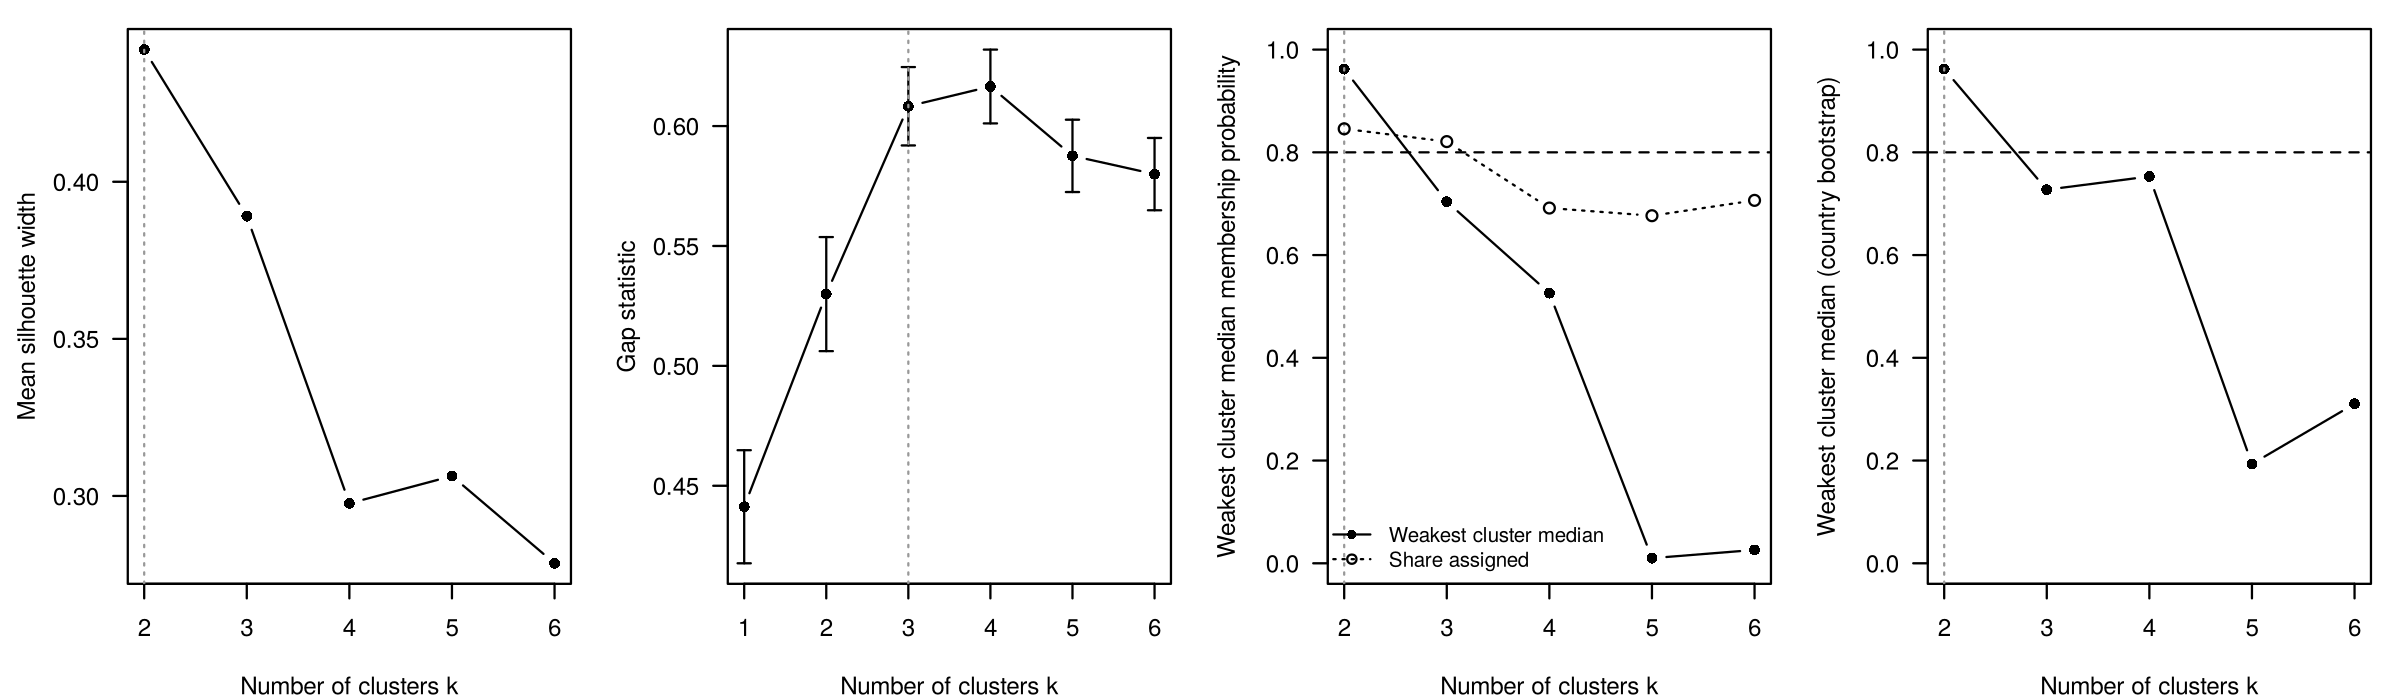
\includegraphics[width=\textwidth]{fig3.png}
\caption{Selection of the number of clusters. From left: mean silhouette width; gap statistic with one-standard-error bars; weakest cluster's median membership probability under value perturbation (filled) with the share of countries assigned (open); the same under country bootstrap. Dashed line, the 0.80 rule; dotted vertical, the $k$ each criterion selects.}
\label{fig:k}
\end{figure}

\subsection{The two clusters}

The decomposition into level and shape did what it was designed to do. Cluster membership explains 5.8\% of the variance in level ($R^2_L$ of~\eqref{eq:r2level}), and its adjusted Rand index against level tertiles is 0.04. The two clusters had almost identical median burden in 1990, 7,239 against 7,062 DALYs per 100,000 (Table~\ref{tab:clusters}, Figure~\ref{fig:level}a), and by 2023 stood at 6,853 against 3,589. They differ in trajectory alone.

Cluster 1, which we label stalled, holds 78 assigned countries whose centred trajectory is nearly flat: a median change of $-7.6\%$ over 33 years, with the cardiovascular peak in the mid-1990s (median 1996, interquartile range 1990 to 2011). Forty of its members are in sub-Saharan Africa, 20 in Southeast Asia, East Asia and Oceania, and none in the high-income super region. Cluster 2, sustained decline, holds 92 assigned countries with a median change of $-52\%$ and the peak at the series start. It contains all 36 high-income super region members, 21 of the 29 countries of Central and Eastern Europe and Central Asia, China, and a minority of Latin American and Middle Eastern countries (Table~\ref{tab:region}, Figure~\ref{fig:comp}). Thirty-one countries are unassigned; they include Morocco, Algeria, Viet Nam, Nepal, Iraq, Venezuela, Botswana, Malaysia and Bulgaria, and their median change of $-31\%$ places them between the two groups. Figure~\ref{fig:traj} shows the centred trajectories and the distribution of membership probability by cluster; Figure~\ref{fig:map} maps the assignment.

\begin{table}[t]
\centering\small
\caption{Cluster characteristics, median (interquartile range). Rates are age-standardised DALYs per 100,000; change is 1990 to 2023; interval width is the country mean of the log-scale standard deviation in~\eqref{eq:sd}.}
\label{tab:clusters}
\adjustbox{max width=\textwidth}{\begin{tabular}{lrrrrrrrr}
\toprule
Group & n & Rate 1990 & Rate 2023 & Change (\%) & Peak year & SDI 2023 & Interval width & Membership probability \\
\midrule
Cluster 1: stalled & 78 & 7239 (5525 to 8836) & 6853 (5235 to 8092) & -7.6 (-16.6 to -0.3) & 1996 (1990 to 2011) & 0.52 (0.42 to 0.63) & 0.097 (0.068 to 0.109) & 1.00 (0.98 to 1.00) \\
Cluster 2: sustained decline & 92 & 7062 (5645 to 10372) & 3589 (2176 to 4877) & -52.4 (-60.0 to -43.3) & 1990 (1990 to 1991) & 0.81 (0.73 to 0.86) & 0.035 (0.027 to 0.049) & 1.00 (0.92 to 1.00) \\
Unassigned & 31 & 7520 (6645 to 11576) & 5399 (4478 to 7511) & -31.4 (-34.4 to -24.7) & 1990 (1990 to 1996) & 0.65 (0.59 to 0.70) & 0.046 (0.034 to 0.098) & 0.43 (0.34 to 0.59) \\
\bottomrule
\end{tabular}
}
\end{table}

\begin{figure}[t]
\centering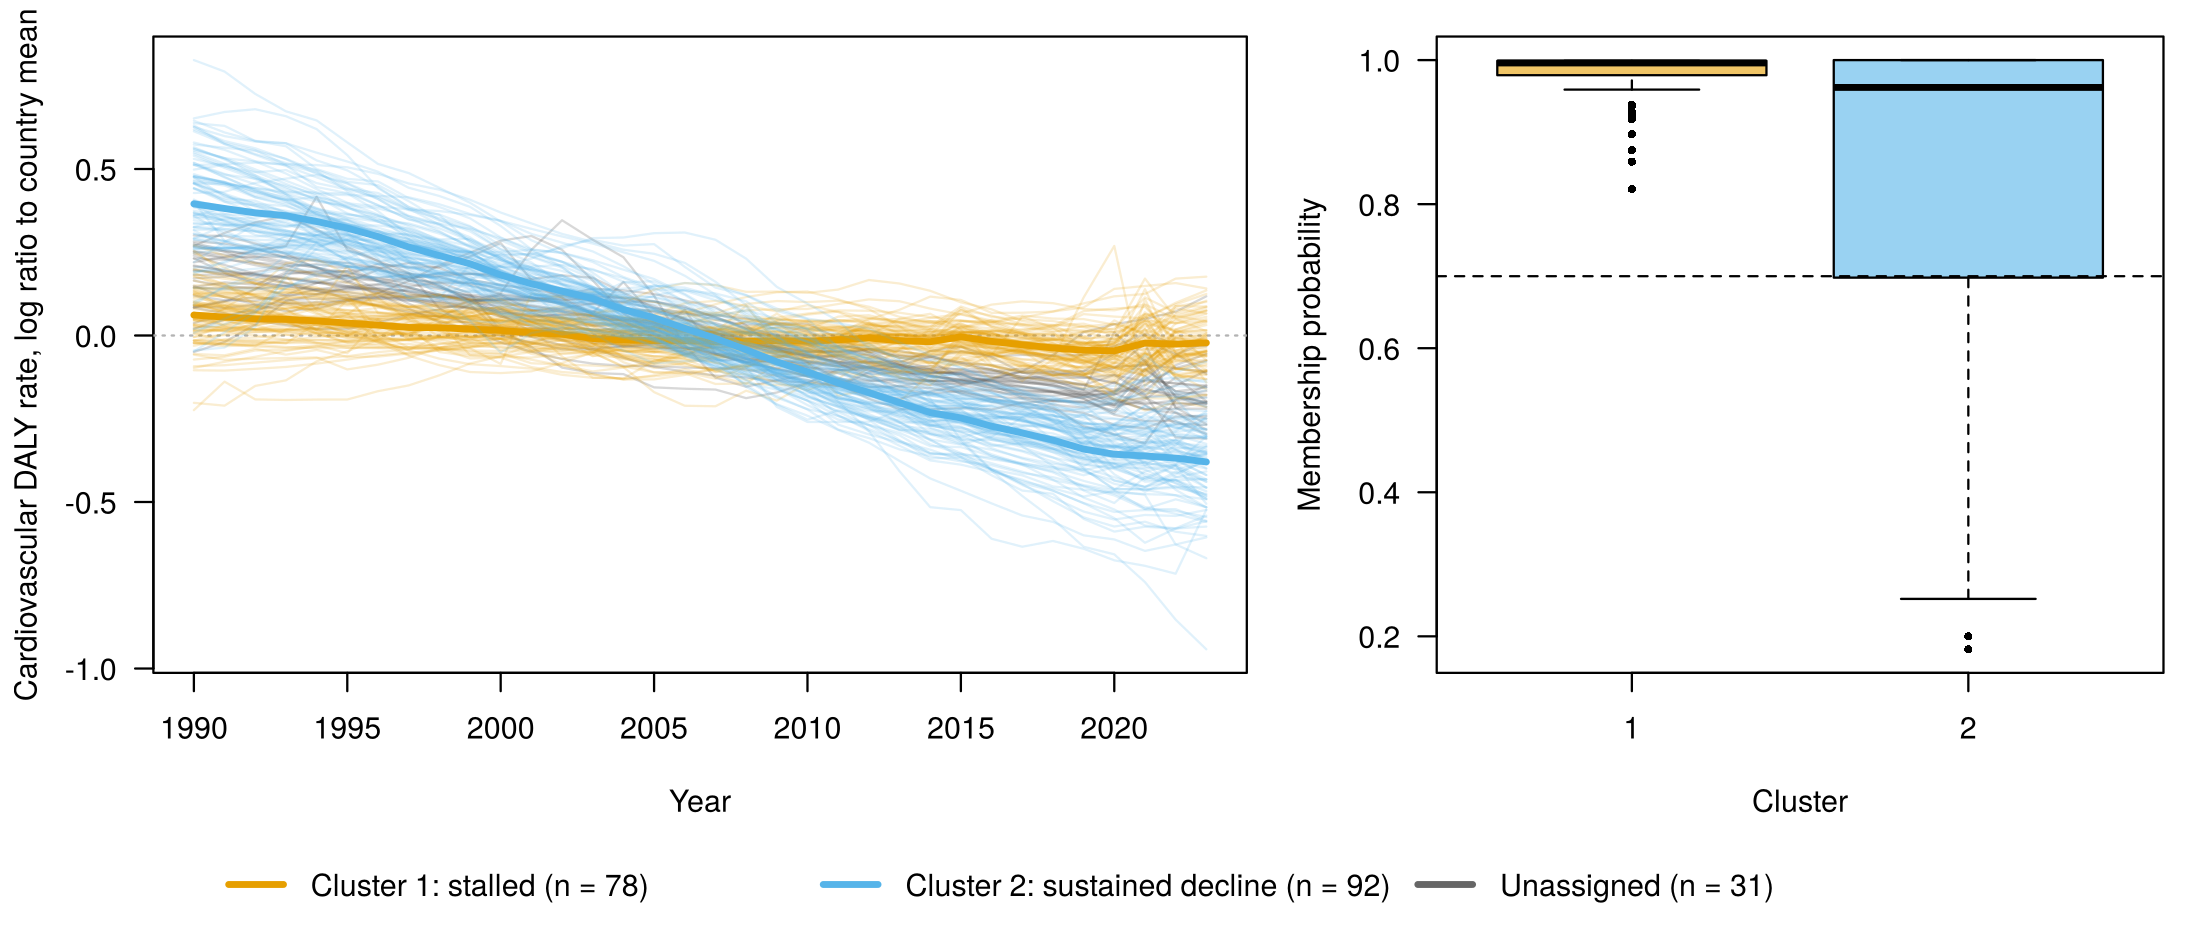
\includegraphics[width=\textwidth]{fig1.png}
\caption{Centred cardiovascular DALY trajectories by cluster (left) and the distribution of membership probability by cluster (right). Thin lines are individual countries, thick lines cluster means, grey lines unassigned countries. The dashed line marks the 0.70 assignment threshold.}
\label{fig:traj}
\end{figure}

\begin{figure}[t]
\centering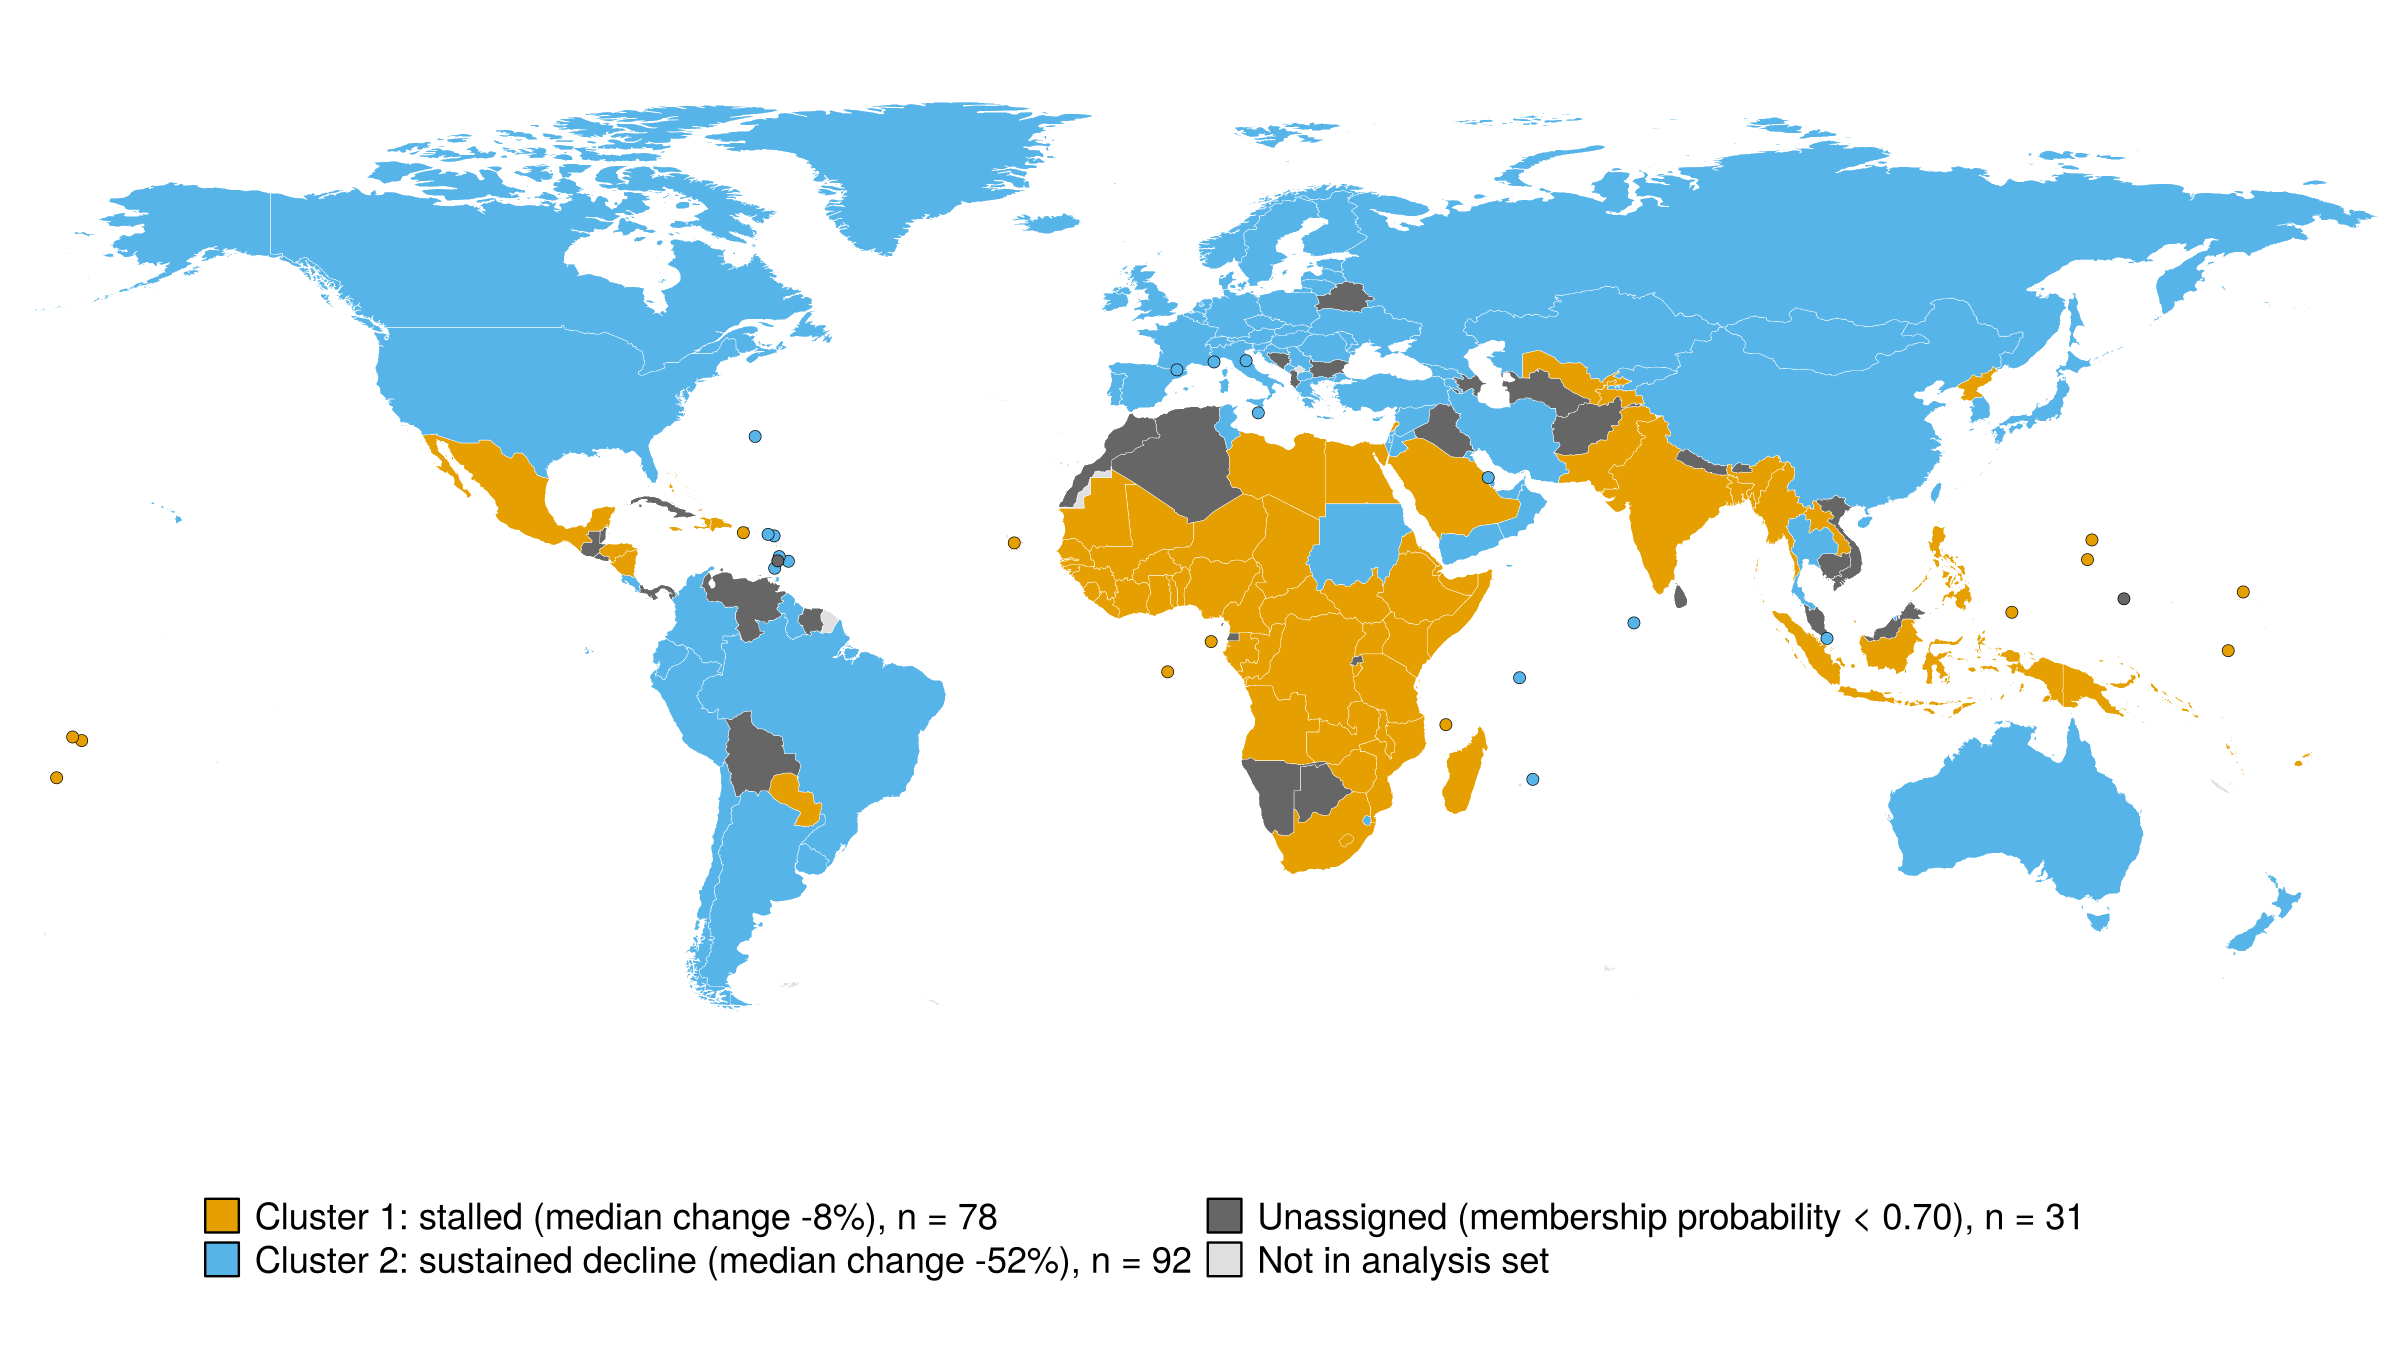
\includegraphics[width=\textwidth]{fig2.png}
\caption{Cluster membership for 201 countries. Orange, stalled; blue, sustained decline; dark grey, unassigned (membership probability below 0.70); light grey, not in the analysis set. Small island states are drawn as points.}
\label{fig:map}
\end{figure}

\begin{table}[t]
\centering\small
\caption{Membership by GBD super region.}
\label{tab:region}
\adjustbox{max width=\textwidth}{\begin{tabular}{lrrrr}
\toprule
Super region & Cluster 1: stalled & Cluster 2: sustained decline & Unassigned & Total \\
\midrule
Central Europe, Eastern Europe and Central Asia &  2 & 21 &  6 &  29 \\
High income &  0 & 36 &  0 &  36 \\
Latin America and Caribbean &  9 & 15 &  9 &  33 \\
North Africa and Middle East &  4 & 13 &  4 &  21 \\
South Asia &  3 &  0 &  2 &   5 \\
Southeast Asia, East Asia and Oceania & 20 &  6 &  5 &  31 \\
Sub-Saharan Africa & 40 &  1 &  5 &  46 \\
Total & 78 & 92 & 31 & 201 \\
\bottomrule
\end{tabular}
}
\end{table}

\begin{figure}[t]
\centering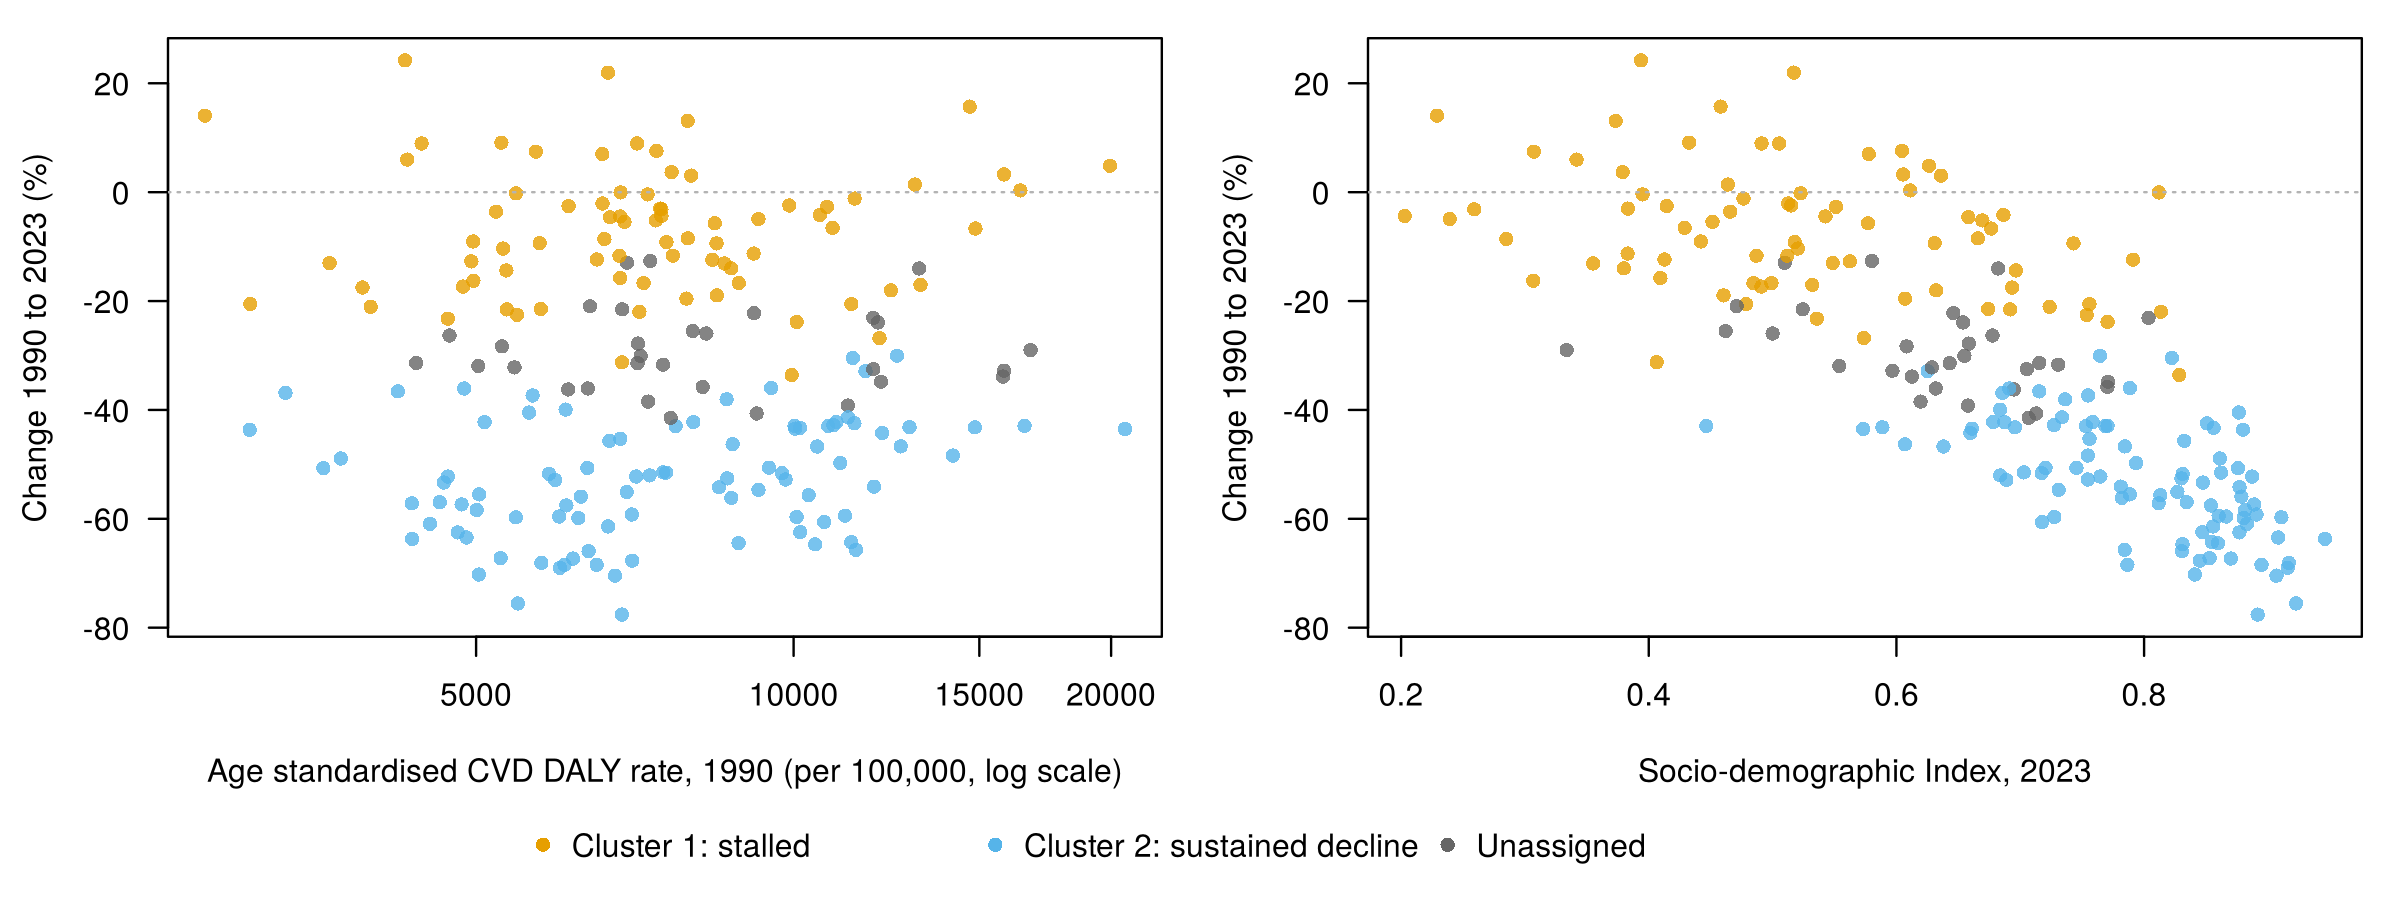
\includegraphics[width=\textwidth]{fig4.png}
\caption{Change in age-standardised cardiovascular DALY rate, 1990 to 2023, against the 1990 rate on a log scale (left) and against the 2023 Socio-demographic Index (right), coloured by cluster. The clusters are indistinguishable on the horizontal axis of the left panel and separate only on change.}
\label{fig:level}
\end{figure}

\begin{figure}[t]
\centering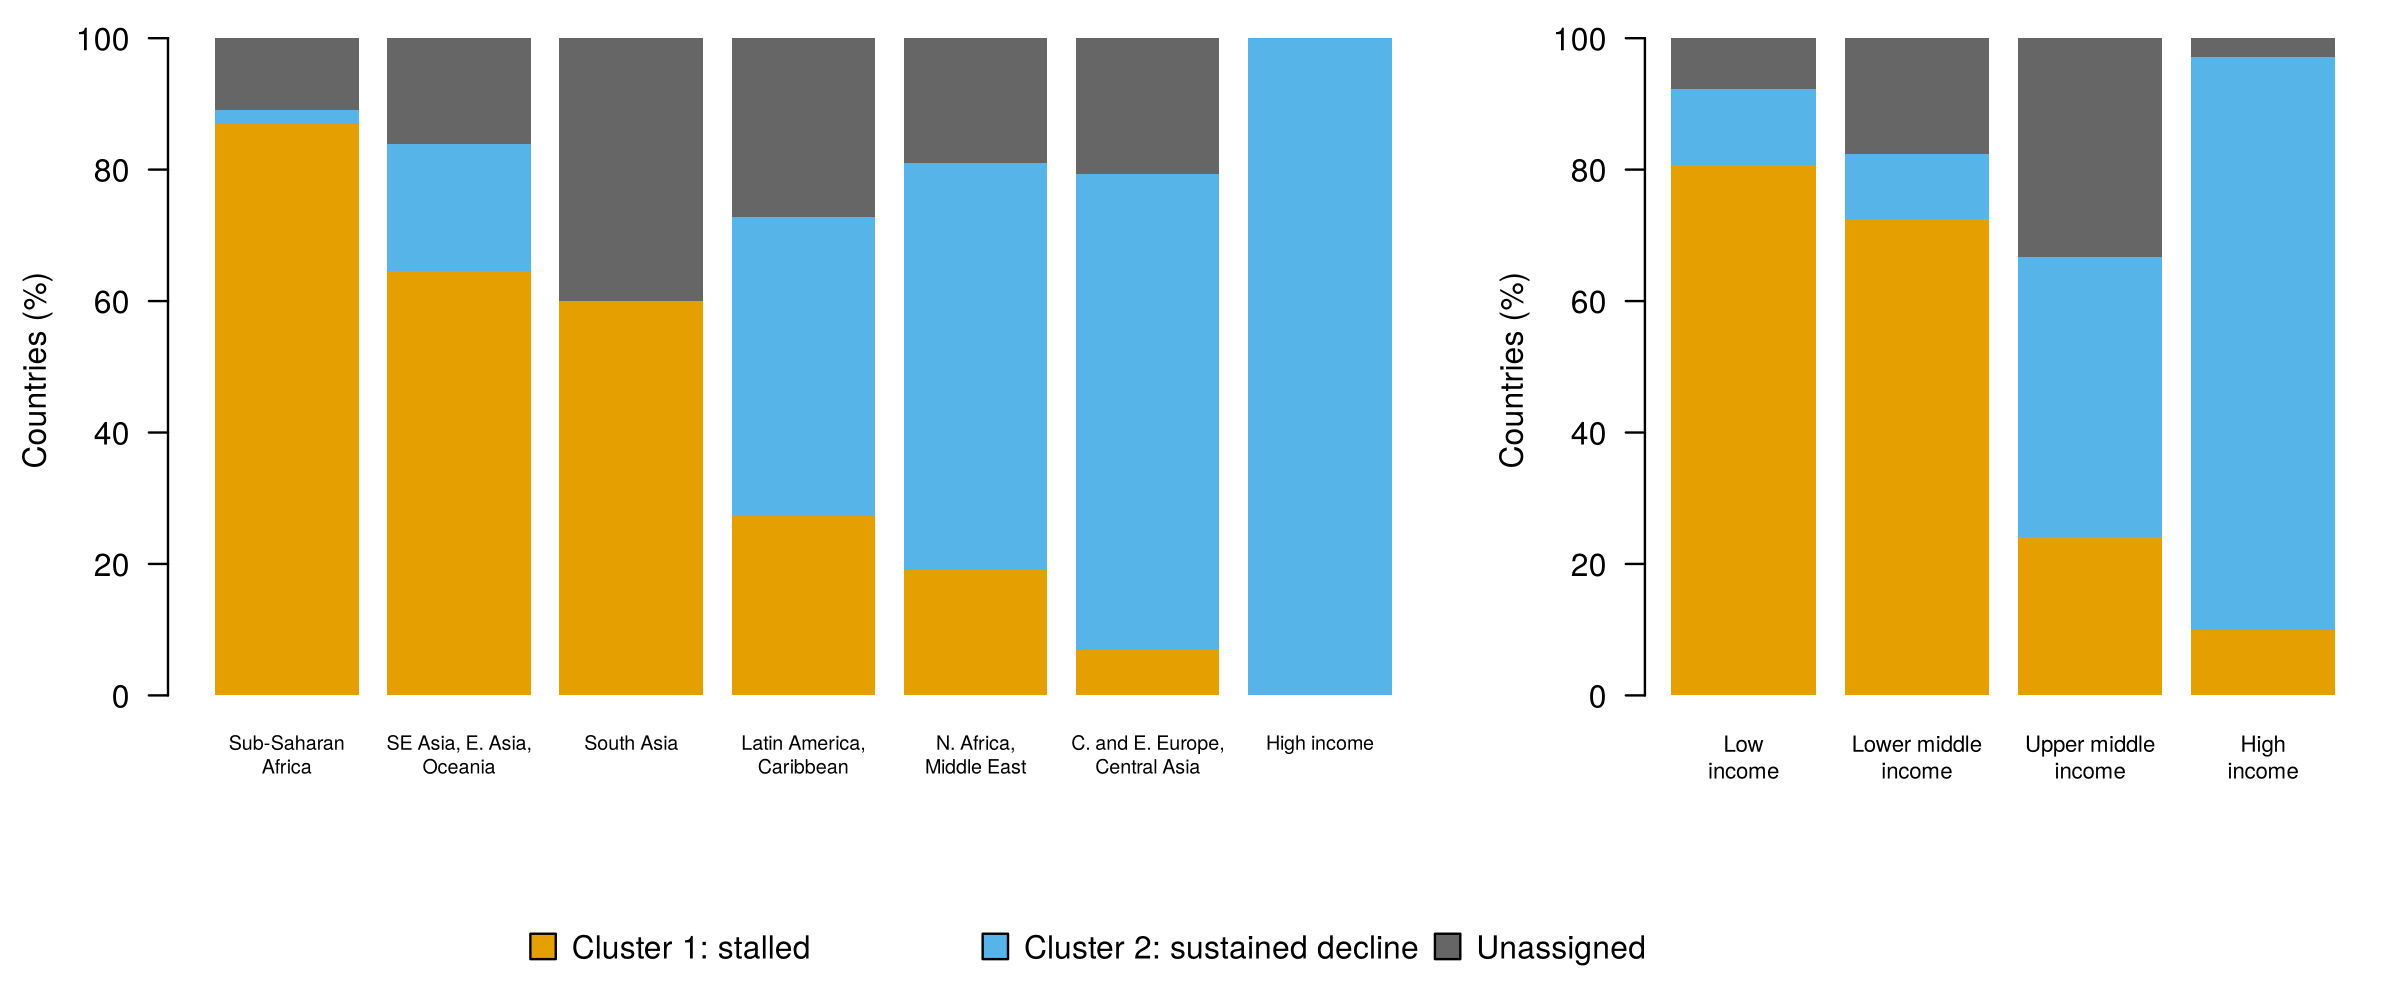
\includegraphics[width=\textwidth]{fig5.png}
\caption{Composition of clusters by GBD super region (left) and World Bank income group (right).}
\label{fig:comp}
\end{figure}

\subsection{Attribution}

Membership is spatially coherent. Moran's I on six-nearest-neighbour weights is 0.56 for the stalled indicator (and, with two clusters, for its complement), and no permutation of 999 reached the observed value; the statistic moves only between 0.53 and 0.58 as the number of neighbours is varied from four to ten (Supplementary Table S4). Development explains about half of the partition: a logistic model of decline versus stalled on SDI alone has McFadden $R^2$ of 0.53, with the odds of the decline cluster rising 5.2-fold per 0.1 unit of SDI. Adding super region raises $R^2$ to 0.63 and the regional term is significant (likelihood ratio test, $p = 0.0005$; Table~\ref{tab:attr}). Geography adds information beyond development level, which a level-based classification would not have produced.

The interval width adds information too. Added to the SDI only model it is significant ($p = 0.011$), with the odds of the decline cluster falling by a factor of 0.11 for every 0.1 increase in mean log-scale standard deviation: at a given development level, the more a country's series depends on modelling, the more likely it is to be stalled. Added to the model that already contains region, it no longer reaches significance ($p = 0.11$), because interval width is itself strongly regional (Figure~\ref{fig:width}a): the median width is 0.024 in Central and Eastern Europe and Central Asia and 0.107 in sub-Saharan Africa. Region and measurement quality are not separable in these data, and Section~\ref{sec:discussion} returns to what that implies.

\begin{table}[t]
\centering\small
\caption{Attribution of membership (sustained decline versus stalled, assigned countries only). Likelihood ratio tests: SDI versus intercept, $p < 0.0001$; region added to SDI, $p = 0.0005$; interval width added to SDI, $p = 0.011$; interval width added to SDI and region, $p = 0.11$.}
\label{tab:attr}
\adjustbox{max width=\textwidth}{\begin{tabular}{lrrrr}
\toprule
Model & Deviance & df & AIC & McFadden R2 \\
\midrule
Intercept only & 234.5 & 169 & 236.5 & 0.000 \\
SDI & 111.0 & 168 & 115.0 & 0.527 \\
SDI + super region &  87.1 & 162 & 103.1 & 0.629 \\
SDI + interval width & 104.5 & 167 & 110.5 & 0.554 \\
SDI + super region + interval width &  84.5 & 161 & 102.5 & 0.640 \\
\bottomrule
\end{tabular}
}
\end{table}

The multinomial model over all 201 countries confirms the reading of the unassigned class as countries in transition rather than noise (Figure~\ref{fig:multinom}). SDI alone gives McFadden $R^2$ of 0.36 and super region adds significantly ($p = 0.002$). The predicted probability of being unassigned rises from near zero at low SDI to a peak of 0.26 at SDI 0.6, exactly where the stalled and decline curves cross, and falls again above 0.8. The framework declines to place countries at the point where the two-shapes are least distinguishable, which is what an honest classifier should do.

\begin{figure}[t]
\centering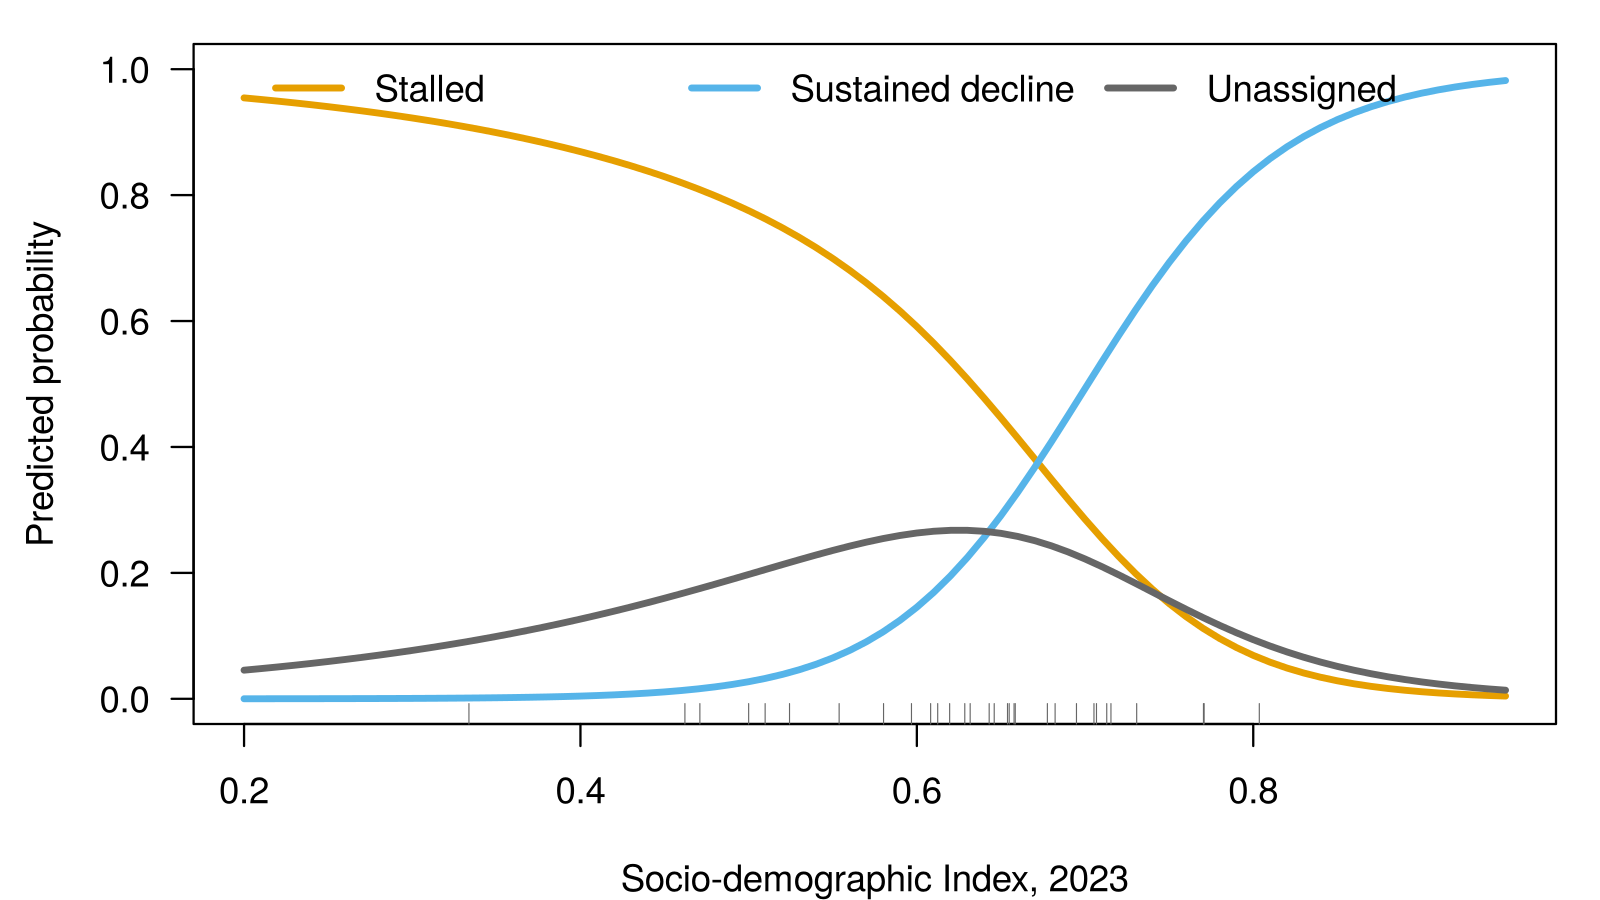
\includegraphics[width=0.7\textwidth]{fig8.png}
\caption{Predicted probability of each membership outcome across the Socio-demographic Index from the multinomial model on SDI alone. Ticks on the horizontal axis mark the SDI of the 31 unassigned countries.}
\label{fig:multinom}
\end{figure}

\subsection{Robustness}

The partition survives every check that the data allow (Table~\ref{tab:robust}, Figure~\ref{fig:robust}). On age-standardised death rates in place of DALYs, all three criteria return the same $k$ as on DALYs, 165 countries are assigned, and among the 156 assigned in both analyses the adjusted Rand index is 1.00: not one country moves between the stalled and decline clusters. The nine countries assigned on DALYs but not on deaths, and the nine assigned on deaths but not on DALYs, are all near the threshold in one measure and all retain the same cluster label. The stalled trajectory is not an artefact of combining mortality and disability.

On the 2000 to 2023 window, all three criteria select two clusters and 188 countries are assigned, the larger number reflecting the smaller spread of trajectory shapes over a shorter window. All 36 high-income countries remain in the decline cluster. The slowdown is real but not a cluster: the median annual change in the high-income super region fell from $-3.5\%$ over 2000 to 2010 to $-1.7\%$ over 2013 to 2023, visible as a flattening of the blue mean in Figure~\ref{fig:robust}b, yet it did not separate those countries from the rest of the decline group. The late-stalling hypothesis of a third trajectory type among wealthy countries is not supported by GBD 2023 at the resolution of this analysis. Of the 31 countries unassigned over the full window, 22 are assigned over the shorter one, ten to stalled and twelve to decline; among countries assigned in both windows the adjusted Rand index is 0.98.

\begin{table}[t]
\centering\small
\caption{Robustness of the primary partition. Agreement is the adjusted Rand index with the primary assignment over countries assigned in both analyses. The narrow half analysis uses the 101 countries with mean interval width below the median.}
\label{tab:robust}
\adjustbox{max width=\textwidth}{\begin{tabular}{lrrrrrr}
\toprule
Analysis & k (silhouette) & k (gap) & k (stability) & Weakest median p at k = 3 & Assigned & ARI with primary (jointly assigned) \\
\midrule
DALYs 1990 to 2023 (primary) & 2 & 3 & 2 & 0.70 & 170 & 1.000 \\
Deaths 1990 to 2023 & 2 & 3 & 2 & 0.66 & 165 & 1.000 \\
DALYs 2000 to 2023 & 2 & 2 & 2 & 0.44 & 188 & 0.976 \\
DALYs, narrowest half of intervals (n = 101) & 2 & 1 & 3 & 0.85 &  72 & 0.414 \\
Country bootstrap instead of value perturbation & 2 & 3 & 2 & 0.73 & 177 & 1.000 \\
\bottomrule
\end{tabular}
}
\end{table}

\begin{figure}[t]
\centering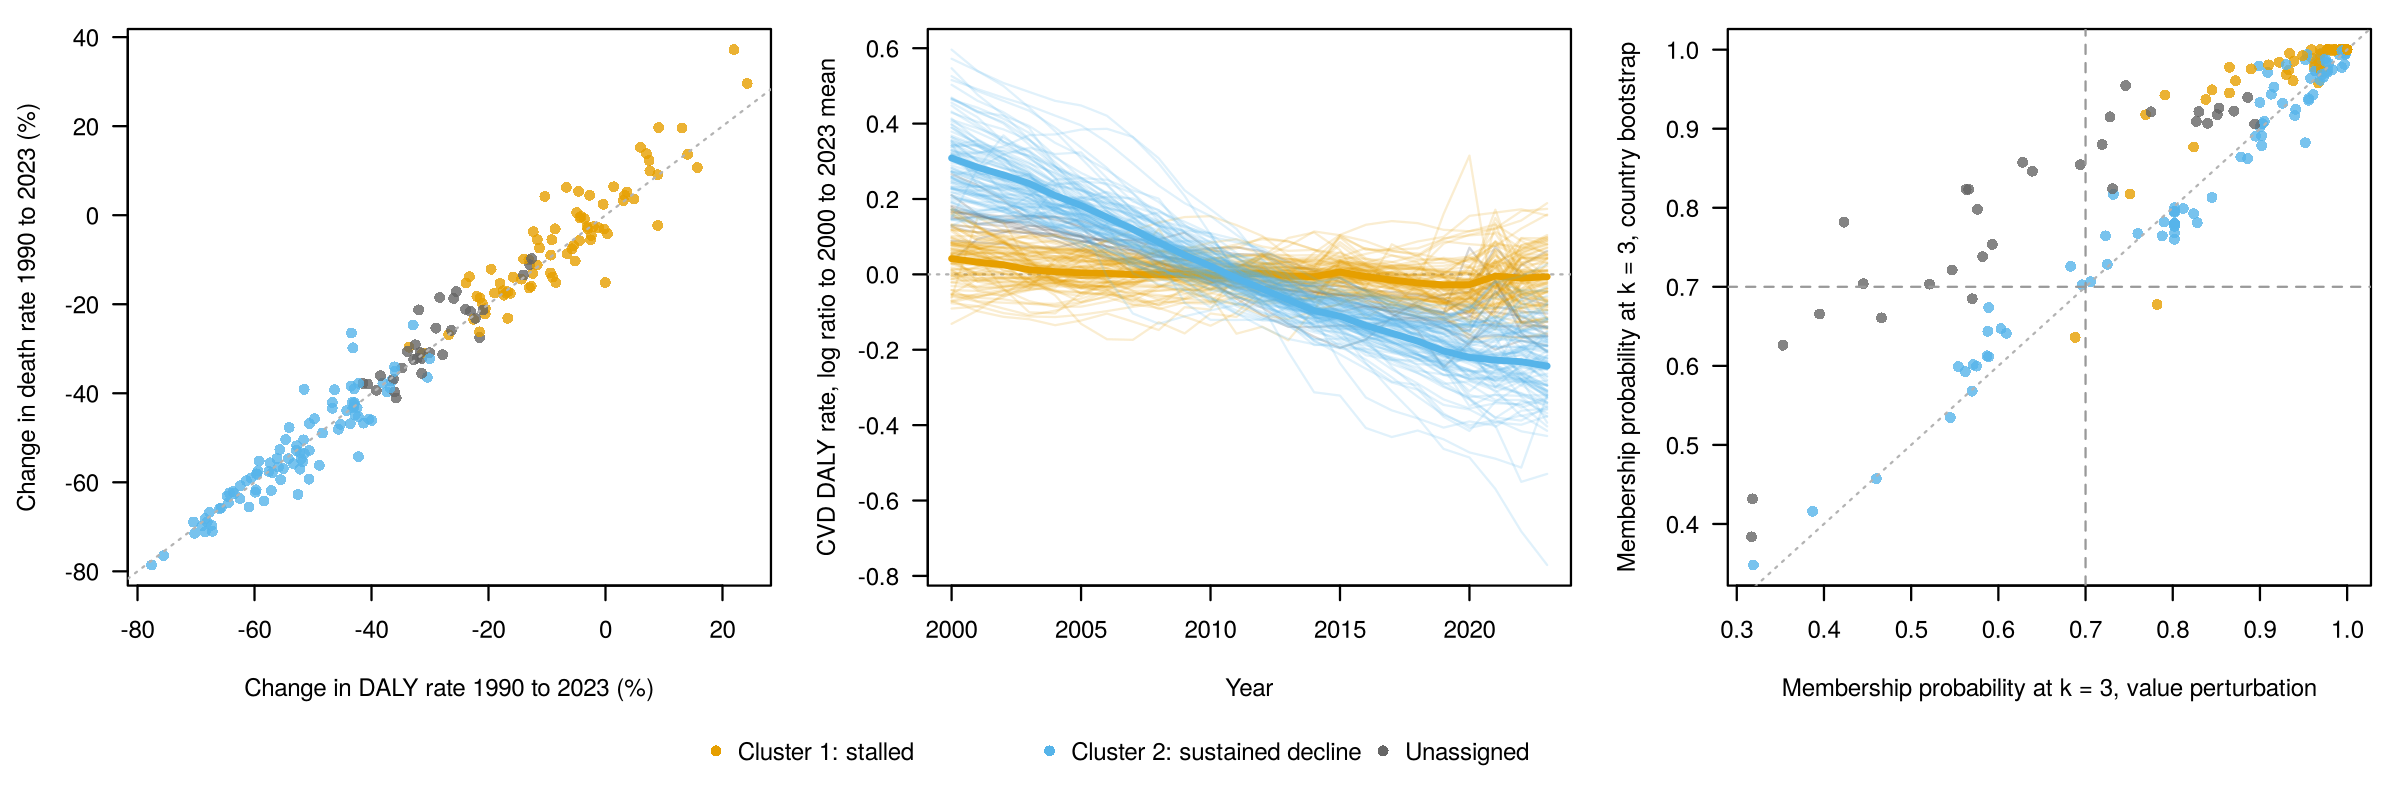
\includegraphics[width=\textwidth]{fig6.png}
\caption{Robustness. (a) Change in death rate against change in DALY rate, 1990 to 2023, coloured by the primary cluster. (b) Centred DALY trajectories over 2000 to 2023, coloured by the window analysis cluster. (c) Membership probability at $k = 3$ under country bootstrap against value perturbation, coloured by the primary cluster; dashed lines at 0.70.}
\label{fig:robust}
\end{figure}

Varying the two tuning constants changes counts, not conclusions. The stability rule $\pi$ selects $k = 2$ for every value from 0.75 to 0.90; at $\pi = 0.70$ it admits $k = 3$, because the weakest cluster at $k = 3$ sits exactly on that boundary (median 0.70), which is why we set the rule above the assignment threshold rather than equal to it. The assignment threshold $\tau$ moves the number of unassigned countries from 24 at $\tau = 0.60$ to 53 at $\tau = 0.90$ without changing the label of any assigned country, since labels come from the reference partition and $\tau$ only gates reporting. We recommend reporting the full membership distribution so that readers can apply their own threshold.

\subsection{What the best-measured countries show}

Restricting the analysis to the 101 countries with mean interval width below the median changes the picture in an instructive way (Figure~\ref{fig:width}c, Table~\ref{tab:robust}). The subset is not representative: it holds 28 of the 29 countries of Central and Eastern Europe and Central Asia, 30 of 36 high-income countries, 29 of 33 in Latin America and the Caribbean, and one country in sub-Saharan Africa. On this subset the uncertainty aware rule selects three clusters, each with median membership above 0.85, where the gap statistic finds no structure at all. The three shapes are the former Soviet and Eastern European rise and fall, with 22 of its 29 members from that super region; the high-income steady decline, with 20 of its 26 from that super region; and a stalled shape of 16 countries, eleven of them in Latin America and the Caribbean, including Mexico, Guatemala, El Salvador, Nicaragua, Paraguay, Venezuela and the Philippines.

Two conclusions follow. The stalled trajectory exists among well-measured countries, so it is not purely a modelling artefact, though among well-measured countries it is a Latin American and Pacific phenomenon rather than an African one. And the pooled analysis loses structure: the Eastern European hump, which the global solution absorbs into the decline cluster, is a distinct and stable shape once the wide-interval series that dominate the pooled variance are removed. Agreement between the subset solution and the primary partition restricted to the same countries is only 0.41 by adjusted Rand index, because the subset splits the primary decline cluster in two.

\begin{figure}[t]
\centering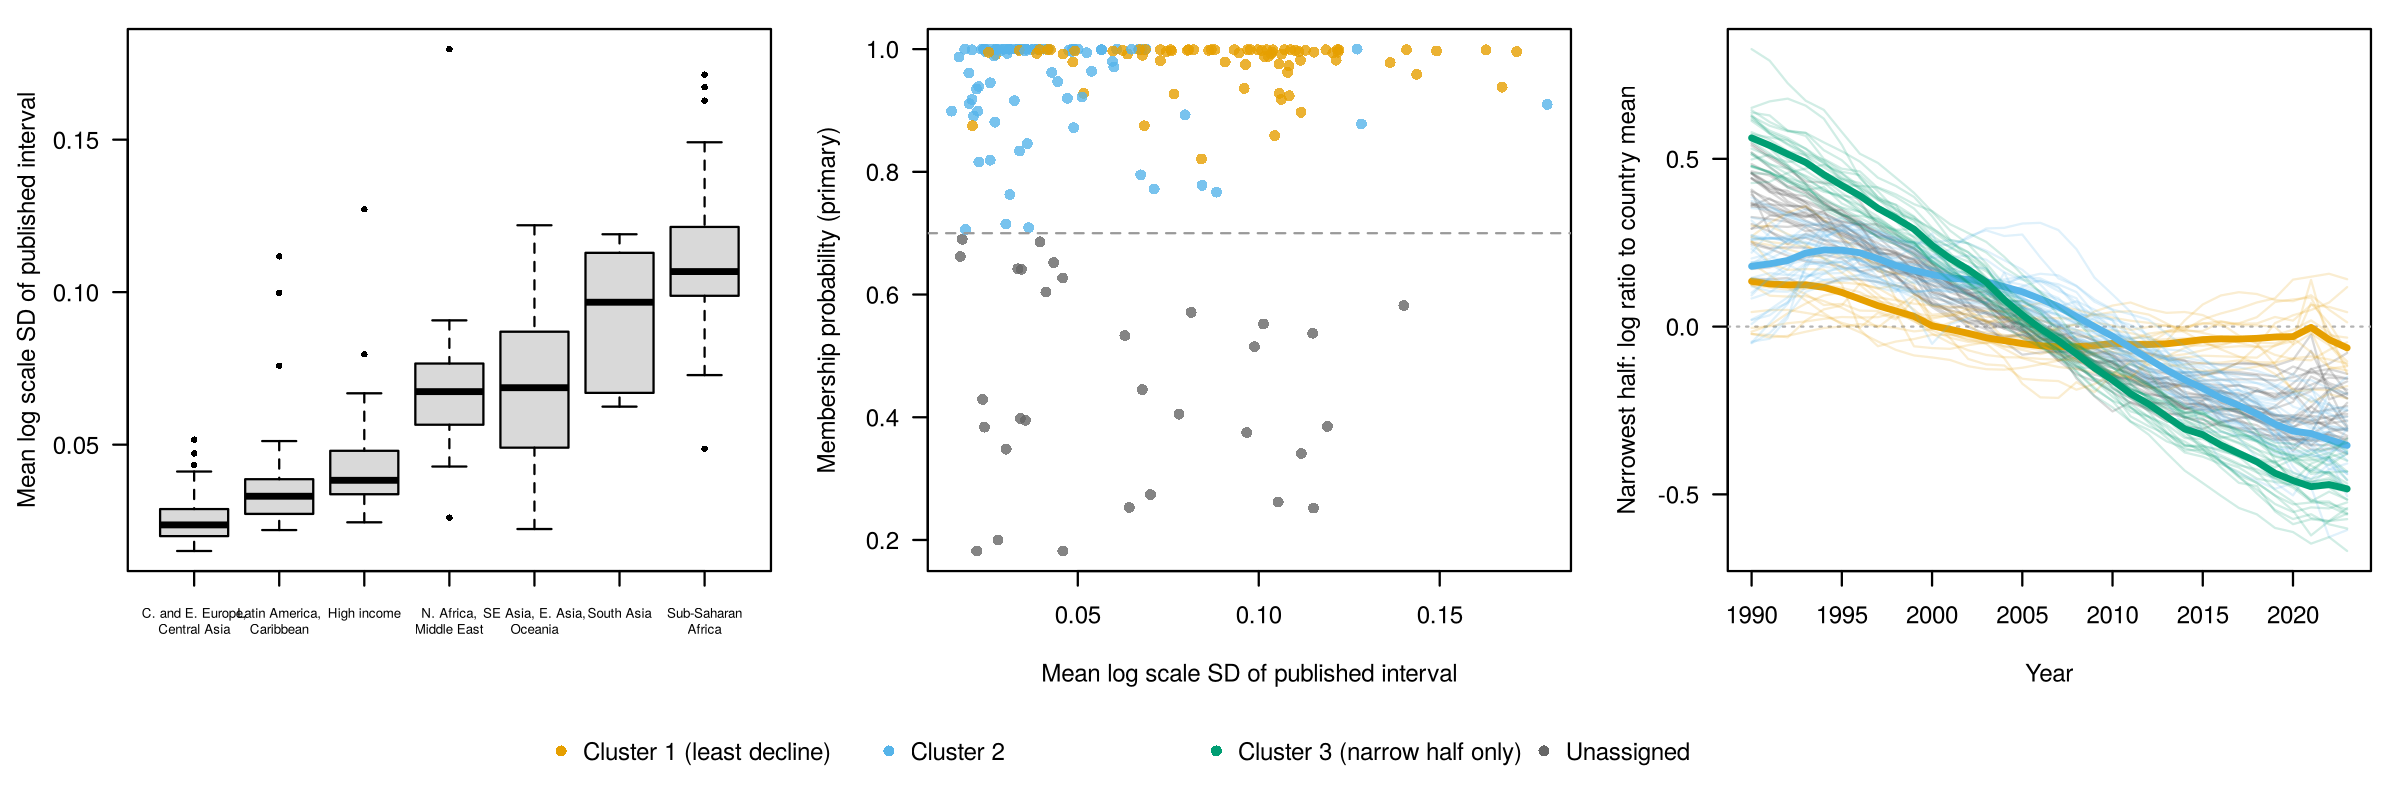
\includegraphics[width=\textwidth]{fig7.png}
\caption{Measurement quality. (a) Mean log-scale standard deviation of the published interval by super region. (b) Interval width against membership probability in the primary analysis. (c) Centred trajectories for the 101 countries with the narrowest intervals, coloured by the three-cluster solution found on that subset; green is the third cluster that appears only here.}
\label{fig:width}
\end{figure}

\section{Discussion}\label{sec:discussion}

\subsection{What the framework changes}

The case study turns on one comparison. A standard, well-regarded criterion for the number of clusters recommended three groups of countries. Perturbing the estimates within their own published uncertainty showed that the third group could not hold its members, and resampling countries instead of values reached the same verdict. A reader of the conventional analysis would have been told that a third cardiovascular trajectory type exists among the world's countries; a reader of this one is told that the data support two, that 31 countries cannot be placed between them, and that those 31 sit at the development level where the two-shapes are least distinguishable. The second account is less tidy and more honest, and we think it is the one that should be standard for any clustering of modelled estimates.

The level and shape decomposition earned its place independently. The two clusters began the period with the same burden and ended it a factor of two apart. A classification on level in 1990 would have found nothing; a classification on level in 2023 would have found nearly the same partition as ours but attributed it to magnitude rather than to the divergence in trajectory that produced it. Separating the two also makes the attribution interpretable: SDI explains about half of the partition and geography adds a significant residual, which is a statement about trajectory types rather than about where burden is high.

The comparison of the two resampling schemes is a result in its own right. Hennig's country bootstrap and the value perturbation agree on the number of clusters here and give strongly correlated membership probabilities, which is reassuring for the many analyses that use only the former. They diverge at $k = 4$, where a cluster that is geometrically well separated but made of poorly-measured countries passes the bootstrap and fails the perturbation. That is the case the value scheme exists for, and it is exactly the case a user of modelled estimates needs to catch.

\subsection{What the cardiovascular result does and does not show}

The stalled cluster is dominated by sub-Saharan Africa and South and Southeast Asia, and the decline cluster by the high-income super region and the former Soviet and Eastern European countries. In broad terms this matches the epidemiological picture in the GBD capstones and the cardiovascular collaboration's 2025 report \citep{gbdcvd2025,gbd2023cod}: sustained decline where control of blood pressure, tobacco and acute care matured early, and stagnation where the transition arrived later and prevention has not kept pace. The mid-1990s peak in the stalled cluster and the continued decline to 2023 in the other are consistent with that reading, and so is the reproduction of the partition on death rates, which rules out an explanation through non-fatal burden alone.

The high-income slowdown deserves a careful statement. It is present in GBD 2023: the median annual decline in the high-income super region halved between the 2000s and the 2010s, in line with the vital statistics analyses of \citet{lopez2019} and the demographic review of \citet{dowd2025}. It did not, over either the full window or the 2000 to 2023 window, produce a third trajectory type, because every high-income country slowed together and the group remained more similar to itself than to anything else. A stalling that is uniform within a group is a change in the group's mean trajectory, not a split in membership, and trajectory clustering will not detect it; a method aimed at change points in the cluster mean would.

Two cautions remain, and the second is the substantive finding of the revision. The first is that DALYs combine mortality and disability; the deaths analysis shows the partition does not depend on that choice. The second is that the stalled cluster coincides with the super region whose estimates lean hardest on covariates. The interval width analysis makes this concrete. Stalled countries have intervals three times as wide as decline countries; width predicts stalled membership even at the same development level; and the association disappears only when region is also in the model, because width and region are nearly the same variable in these data. We cannot, from GBD outputs alone, say whether sub-Saharan Africa's stalled trajectory reflects an epidemiological reality or the smoothness of covariate-driven estimates, and we do not think any analysis of GBD outputs alone can. What the framework can do is show the dependence and keep the countries with the widest intervals out of the assigned set when their shape is ambiguous. The well-measured subset does show that a stalled shape exists where measurement is good, but in Latin America and the Pacific rather than Africa, and that the best-measured countries carry a three-shape structure that the pooled analysis flattens. The decisive test, a rerun on countries at four and five stars on GBD's own vital registration rating \citep{gbd2016cod,gbd2023cod}, requires the star ratings, which the access route used here does not expose.

\subsection{Limitations}

The uncertainty propagation uses independent normal perturbations on the log scale with standard deviations taken from the all-ages interval, and ignores the correlation between years that posterior draws carry. Both approximations are imposed by the access route, both are removable, and both are conservative in direction; draw-level replication from the GBD Results Tool is the first item on the revision list. Interval width is a proxy for data density, not a measure of it; it reflects modelling uncertainty of every kind and would be replaced by the published star ratings in a final analysis. The clustering is univariate by design, so the trajectory types are cardiovascular trajectory types, not epidemiological transition types; the framework extends to several causes by concatenating scaled shape vectors, and that extension is planned. The attribution stage uses one covariate and a seven-level region factor; a fuller model would include health system and risk factor covariates and a spatial random effect in place of the fixed region term. The constants $\tau$ and $\pi$ are conventions from the stability literature, not derived quantities, and we report the full membership distribution so readers can apply their own.

\subsection{Implications}

For analysts of GBD and similar modelled outputs, the practical recommendation is short. Report the number of clusters under a stability criterion alongside the geometric ones, perturbing values within their published intervals and not only resampling units. Report a membership probability for every unit and leave units unassigned when their interval permits them to move. Report the width of the interval as a covariate, and treat any cluster that tracks it as provisional until it is reproduced on well-measured units. All of this is cheap: the analysis here runs in about a minute. For the cardiovascular question, the result is a map of where the transition has stalled that comes with an honest account of which countries it cannot place, a demonstration that the high-income slowdown has not yet broken the high-income cluster, and a flag that the African stalled trajectory needs confirmation from registered deaths before it is treated as settled.

\section*{Declarations}

\paragraph{Data availability.} All inputs are public GBD 2023 outputs of the Institute for Health Metrics and Evaluation. The extracted panels, lookup tables and R scripts that reproduce every table and figure are provided as supplementary material.

\paragraph{AI assistance.} Claude (Anthropic) was used in preparing this manuscript for data extraction from the GBD 2023 connector, drafting and executing the R analysis code, generating figures and tables, literature search, and drafting the text. All code was executed in R 4.3.3; all numerical results were produced by that code; every reference was checked against a publisher or repository record before inclusion, and those not yet checked are marked. The author reviewed and revised all outputs and takes responsibility for the content. [Confirm wording against the target journal's policy and reproduce all numbers locally before submission.]

\paragraph{Funding.} None declared. \textbf{Competing interests.} None declared.

\paragraph{Colour convention.} The same colours carry the same meaning in every figure: orange for the stalled cluster, blue for the sustained decline cluster, green for the third cluster of the narrow interval analysis, dark grey for unassigned countries.

\section*{Supplementary material}
Supplementary Table S2 lists all 201 countries with region, income group, SDI, change in DALYs and deaths, peak year, interval width, and cluster and membership probability under the primary, deaths and 2000 window analyses. Table S3 lists the unassigned countries, Table S4 gives Moran's I for four to ten nearest neighbours, Table S5 the sensitivity to the tuning constants, Table S6 the selection diagnostics for every robustness run, and Table S7 the composition of the narrow-interval solution. Section S1 documents the extraction and Section S6 the reproduction steps. The R scripts \texttt{final\_analysis.R} and \texttt{extended\_analysis.R}, the four panels and the two lookup tables reproduce every result.

\bibliographystyle{plainnat}
\bibliography{refs}

\end{document}
